\section{Transactive Energy Standard Design}\label{sec:standard_design}

In the section we focus on the design requirements for a transactive system, as embodied by the TESS platform, and it differs from the ``standard'' transactive system as embodied by previous field deployments. In its full development a transactive energy system is intended to comprise multiple retail-level price discovery systems specifically tailored to the needs of the utilities and customer where they are deployed.  This implies the need for a high degree of flexibility regarding which kinds of prices are discovered, the timing and physical extent of the retail market systems, the types of devices that participate, and the manner in which transactions are settled.

\subsection{Prices Discovery Mechanisms}

Most transactive systems are currently designed to discover energy prices in \$/MW.h, i.e., bid quantities are measured in MW.  The analogy to wholesale energy market is obvious, insofar as it was designed to mitigate distribution constraints. Indeed it was this analogy that made the Olympic project \cite{hammerstrom_2008} so easy to realize why it is the basis of what is often referred to now as the ``standard'' transactive system design.

However, the bidding strategies for some resources can be difficult to design for an energy-only retail market.  For example, in the Olympic project, diesel generators had a very complex bidding strategy because of the 100 hour annual maximum run-time license.  In addition, there are potential issues with incentive compatibility when using thermostatic devices if consumers are given too much control over the bidding strategy \cite{Somani???}. Thus high degrees of automation not only ensured strong demand response resource participation, it also protected against strategic bidding practices that could undermine the design objectives of the mechanism.

Although it was not initially needed by HCE, TESS is designed to support up to three distinct price discovery mechanisms simultaneously, i.e., energy prices (\$/MW.h), storage prices (\$/MW.h$^2$), and ramping prices (\$/MW). At the time of this writing, these are beyond scope of the standard transactive design, and it is not clear how and whether storage and ramping price discovery will be as effective at efficiently dispatch resources as energy price discovery is. There are projects planned that will explore these questions in the coming years.

\subsection{Time and size scales}

The double clock auction mechanism is also a key feature of the standard transactive system design.  The auction used on most extant transactive projects has important limitations that TESS seeks to overcome in its design.  This includes the inability to clear resources that can act significantly faster than the auction interval, which is typically 5 minutes. TESS allows a utility-specified market clearing interval, although the default is still 5 minutes.  It is also difficult, if not impossible, to reveal any forward knowledge through the double auction  mechanism. To address these problems, the TESS design includes an order-book mechanism that accept to types of bids, i.e., market orders, and limit orders.  A market order allows a resource to immediately dispatch at the current price, whatever it is.  A limit order allows a resource to be reveal its dispatch capabilities for any future time interval, contingent on a suitable ask or offer price.  Here too, the HCE did not need to address any of these shortcomings and the Basalt project does not use a non-standard market-clearing interval or an order-book clearing mechanism.

The physical scaling of transactive system can be a difficult design and implementation problem for utilities, although usually it is not a problem. For example, in the Columbus demonstration project \cite{Widergren2014} the standard transactive system was deployed on 4 feeder without significant changes to the implementation.  However, the Pacific Northwest project \cite{hammerstrom_2015} encountered number of important market design and operation issues that emerged due the need to coordinate the dispatch retail resources across 11 utilities in a region that does not have a restructured electricity market.  In the case of HCE, the system operates in a well-defined wholesale environment and none of these issues emerged. Therefore the TESS platform has yet to be evaluated in this regard.

\subsection{Types of participating devices}

In the standard design piloted by the Olympic project, thermostat heating/cooling devices, diesel generators, micro-turbines, white goods appliance, and municipal water pumping systems were the principal resources that could place asks and offers in the retail market.  At the time, these were typical of the devices the utilities hoped to dispatch using a retail real-time energy price.  More recently, new types of flexible resources figure prominently in utility distribution system operations.  Among these rooftop photo-voltaics, battery energy storage, and electric vehicle chargers have emerged as a primary concern. HCE energy plans to test all three of these resources using TESS as well as eventually including heat-pump heating/air-conditioning and heat-pump water heaters.

\subsection{Settlement mechanisms}

Several settlement systems have been demonstrated in previous transactive systems, including a side-payment mechanism \cite{hammerstrom_2008} and a regulator-approved tariff \cite{Widergren2014}. TESS proposed two additional settlement systems based on tokens.  

The first uses an implied Shapley value calculation, where a certain number of tokens are issued each month by the utility based on the expected value of the total welfare surplus from operations.  Customers then participate in the transactive system using these tokens, and the total surplus at the end of the billing cycle is used to assign a value to the tokens, which is then used to compute individual bill credits.  

However, uncertainty regarding whether such a settlement mechanism might run afoul of new federal securities regulations required the development of a second financially equivalent mechanism wherein customer participate in the local currency and at the end of the billing cycle, all participants are charged a share of the total cost of operating the system in proportion to their net earnings under the transactive system. HCE has elected to use the latter system as part of a rebate system under the existing flexible demand tariff. \textcolor{red}{MLA: please confirm that I described this correctly and fix it if not.} There remains an open question regarding whether these settlement mechanisms would be perceived as equivalent by customers. This question cannot be evaluated until both mechanisms have been tested at sufficiently large scale, which is beyond the scope of the HCE field test.

\textcolor{red}{MLA: We need a section which described the `pure' transactive system. I am thinking that it might make sense to merge this section with the introduction as the `pure' design is not overly complicated (`market-based coordination of customer appliances'). If we wanna be more comprehensive, we can keep it as a separate section but should be aware of not repeating too much between this section and the intro.}

Described in detail in Hammerstrom et al 2007. Main mechanism is direct bidding etc.

TE 2.0, prices from devices
\begin{itemize}
    \item Market-based coordination
    \item Digitally-enabled devices
    \item Market platform
    \item Buyers submit bids
    \item Sellers submit offers
    \item Transactions occur, details vary depending on market design/auction design
    \item Market-clearing price serves as signal for autonomous device control and price-based dispatch; devices algorithmically change settings
    \item Combination of physical grid reality as a constraint + market coordination of Qs=Qd yields simultaneous physical balance and economic efficiency with minimal user information/respect for data privacy
\end{itemize}

PNL 2007 summarize, Dave dissertation

\begin{figure}[h]
\centering
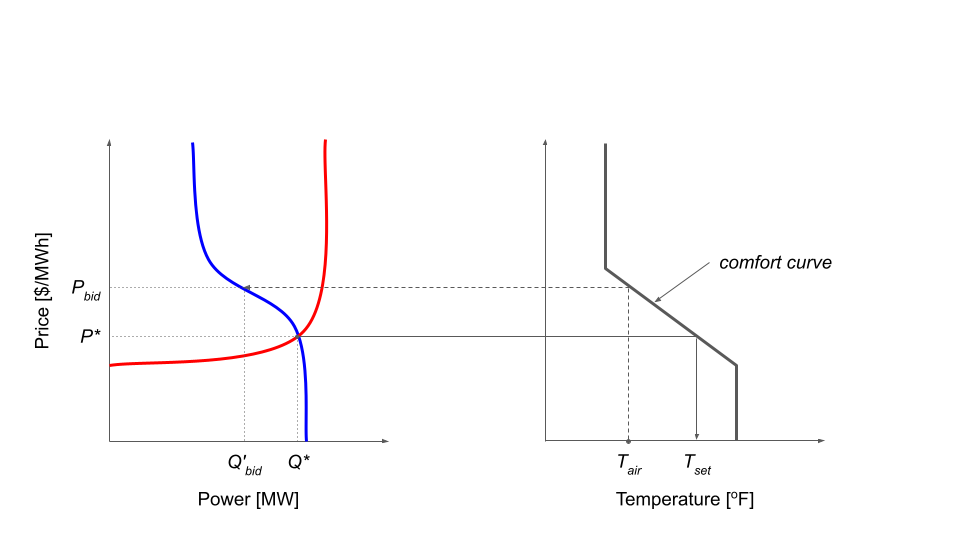
\includegraphics[scale=0.4]{images/TE_DA.png}
\caption{Transactive Double Auction Design}
\label{fig:Transactive_DA}
\end{figure}


too risky for utilities to implement
